% *********************************************************************
% © 2016–2023 Jeremy Sylvestre
%
% Permission is granted to copy, distribute and/or modify this document
% under the terms of the GNU Free Documentation License, Version 1.3 or
% any later version published by the Free Software Foundation; with no
% Invariant Sections, no Front-Cover Texts, and no Back-Cover Texts. A
% copy of the license is included in the appendix entitled “GNU Free
% Documentation License” that appears in the output document of this
% PreTeXt source code. All trademarks™ are the registered® marks of
% their respective owners.
%
% *********************************************************************
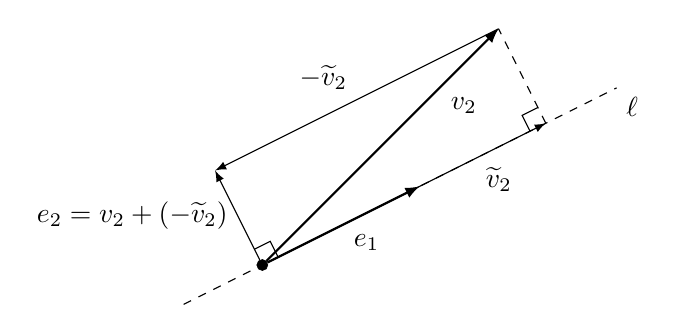
\begin{tikzpicture}[
	point/.style={circle,draw,very thin,fill,inner sep=0pt,minimum size=4pt},
	vector/.style={-latex},
]

	\node[point] at (0,0) (o) [label=below:{$\zerovec$}] {};
	\draw[dashed] (-1,-0.5) to node[below right,at end] {$\ell$} (4.5,2.25);
	\draw[vector,thick] (o) to node[below right,near end] {$\uvec{v}_2$} (3,3);
	\draw[vector,thick] (o) to node[below right] {$\uvec{e}_1$} (2,1);
	\draw[vector] (o) to node[below right,near end] {$\widetilde{\uvec{v}}_2$} (3.6,1.8);
	\draw[vector] (3,3) to node[above left] {$-\widetilde{\uvec{v}}_2$} (-0.6,1.2);
	\draw[vector] (o) to node[left] {$\uvec{e}_2 = \uvec{v}_2 + (- \widetilde{\uvec{v}}_2)$} (-0.6,1.2);
	\draw[dashed] (3.6,1.8) to (3,3);
	\draw (0.2,0.1) to (0.1,0.3) to (-0.1,0.2);
	\draw (3.4,1.7) to (3.3,1.9) to (3.5,2);

\end{tikzpicture}
